\textbf{The simulation gives two plausible estimates for
the time-since-collision, with $TSC_0 = \giga \text{yr}$ and $TSC_1 = \giga
\text{yr}$}. The presence of the radio relic, in conjunction with a
depression in the X-ray surface brightness shown in M11, strongly suggest
that El Gordo is a post-collision system. 
Based on section \ref{sec: positionprior}, we have come up with an estimate for the
likely position of the NW radio relic based on the two inferred TSC. 
We summarize the realizations for the two possible scenarios with the
polarization prior applied in Figure \ref{fig: positionprior}, while we
leave the results from the default prior in Appendix \ref{app: merger_scenarios}.
The green and blue distributions on upper panel of Figure \ref{fig:
positionprior} denoted the lower bound for the location of the NW
subcluster. 
While on the lower panel of Figure \ref{fig: positionprior}, the blue and
green curves denote the approximate upper bound on the location of the
relic. After taking into the uncertainty in the time evolution of the velocities,
the position of the observed relic favors the outgoing scenario.  

Other
uncertainties arise from how we define the reference frame for the calculation. The
uncertainty associated with the two centroids are of the order
of $\sim 0.1 \mega$pc \citep{Jee13} and are relatively unimportant???.  

\begin{figure}
	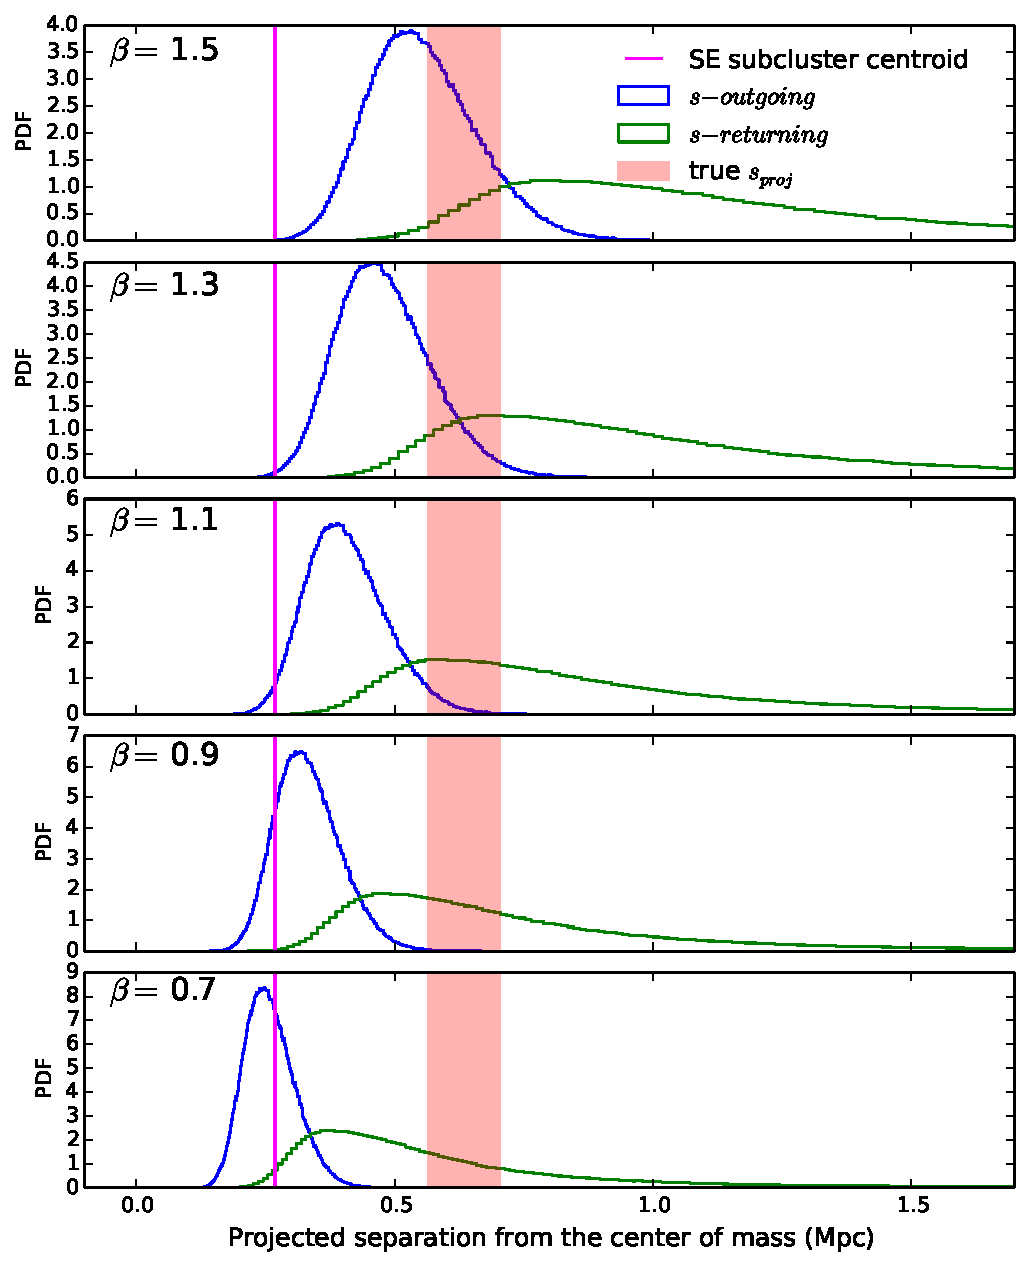
\includegraphics[width=\linewidth]{polar_prior_bounds.pdf}
	\caption{Position of the radio relic based on the estimated minimum
	velocities (upper figure) and the estimated maximum velocities (lower
	figure) \label{fig: positionprior}}
\end{figure}



%Base on the time evolution of radio relic, we speculate that El Gordo has already reached its apoapsis and the two subclusters are heading for another merger.
%%This degeneracy between $TSC_0$ and $TSC_1$ that
%is not resolved by taking the separation constrain from the radio relic. 

%the post-collision estimate of the
%time-since-collision ($TSC_0$), the pre-collision estimate of the
%time-since-collision ($TSC_1$) and the time between collisions ($T$).
%We pick the post-collision time-since-collision estimate ($TSC_0$) of Gyr to be representative of the observed status of El Gordo, instead of the pre-collision time-since-collision estimate ($TSC_1$). While the simulation models both scenarios either the subclusters are approaching each other (incoming) or they have already passed through each
%other and are moving apart (outgoing), the presence of the radio relic rules out the possibility that the two subclusters still have not encountered each other. 
%However, this does not exclude the possibility of having the subcluster
%approaching each other again after reaching apoapsis.  
%%\citet{b9} have reported that the simultaneous optical and near-IR data of
%%AC Her can be fitted by a combination of two blackbodies at 5680 and
%1800\,K, representing, respectively, the stellar and

